\documentclass[11pt]{beamer}

\usetheme{Madrid}
\usecolortheme{default}
\setbeamertemplate{navigation symbols}{}
\setbeamertemplate{footline}[frame number]
\setbeamertemplate{caption}[numbered]

\usepackage[T1]{fontenc}
\usepackage{graphicx}
\usepackage{booktabs}
\usepackage{xcolor}
\usepackage{listings}
\usepackage{amsmath}
\usepackage{textcomp}

\definecolor{codebg}{rgb}{0.95,0.95,0.95}
\lstset{
  basicstyle=\ttfamily\scriptsize,
  backgroundcolor=\color{codebg},
  breaklines=true,
  frame=single,
  columns=fullflexible,
  language=C++,
  showstringspaces=false,
  keywordstyle=\color{blue!70!black}\bfseries,
  commentstyle=\color{gray},
}

\newcommand{\coderef}[1]{{\scriptsize\textcolor{blue!60!black}{\texttt{#1}}}}

\title[Geometric Verification \& Scene Graph Augmentation]{Geometric Verification \&\\ Scene Graph Augmentation}
\subtitle{Assignment 1, Problem 2 --- Understanding COLMAP's SfM Pipeline}
\author{Team [Names]}
\institute{E9-247: Learning for 3D Vision, IISc}
\date{September 24, 2026}

\begin{document}

% ---------------------------------------------------------------------
\begin{frame}
  \titlepage
\end{frame}

% ---------------------------------------------------------------------
\begin{frame}{Topic \& Grounding}
  \small
  \textbf{Task:} validate matched image pairs and build a robust scene graph
  \begin{itemize}\setlength{\itemsep}{1pt}
    \item \textbf{Paper:} Sch\"onberger \& Frahm, \emph{Structure-from-Motion Revisited}, CVPR 2016 --
          Sec.~2.1 \& 4.1
    \item \textbf{Code:} \texttt{colmap/src/colmap/estimators/two\_view\_geometry.\{h,cc\}}
  \end{itemize}
  \vspace{0.15cm}
  \textbf{Five guiding questions we answer, each grounded in code:}
  \begin{enumerate}\setlength{\itemsep}{1pt}
    \item What does H verify vs.\ F/E, and why doesn't a valid H mean ``safe to triangulate''?
    \item Why isn't a single model (just F) enough?
    \item What do $N_H/N_F$ and $N_E/N_F$ actually indicate about the scene?
    \item What is a WTF (watermark) pair, and why does it fool a naive verifier?
    \item With fixed thresholds, how does a borderline pair get resolved?
  \end{enumerate}
  \vspace{0.15cm}
  \textbf{Required experiment (two parts):} real $N_F,N_E,N_H$ across scene types,
  plus a borderline-pair threshold sweep.
\end{frame}

% ---------------------------------------------------------------------
\begin{frame}[fragile]{The Verification Decision Tree (the code, in one slide)}
  \texttt{TwoViewGeometryOptions} defaults --- \coderef{two\_view\_geometry.h:18--111}:
  \begin{center}
  \scriptsize
  \begin{tabular}{lll}
    \toprule
    \texttt{min\_num\_inliers} & $=15$ & floor for any non-degenerate model \\
    \texttt{min\_E\_F\_inlier\_ratio} & $=0.95$ & paper's $\epsilon_{EF}$ \\
    \texttt{max\_H\_inlier\_ratio} & $=0.80$ & paper's $\epsilon_{HF}$ \\
    \texttt{watermark\_min\_inlier\_ratio} & $=0.70$ & WTF border+translation ratio \\
    \texttt{ransac\_options.max\_error} & $=4.0$px & shared by F, E, H \\
    \bottomrule
  \end{tabular}
  \end{center}
  Classification, \coderef{two\_view\_geometry.cc:1148--1207} (calibrated) / \coderef{cc:425--441} (uncalibrated):
  \begin{lstlisting}
fit E, F, H independently (LO-RANSAC, same 4px thresh.)
if E passed and N_E/N_F > eps_EF:
    if N_H/N_E > eps_HF:  config = PLANAR_OR_PANORAMIC
    else:                 config = CALIBRATED
elif F passed:
    if N_H/N_F > eps_HF:  config = PLANAR_OR_PANORAMIC
    else:                 config = UNCALIBRATED
elif H passed:            config = PLANAR_OR_PANORAMIC
else:                     config = DEGENERATE
  \end{lstlisting}
\end{frame}

% ---------------------------------------------------------------------
\begin{frame}{Q1: What does H verify vs.\ F/E?}
  \begin{columns}[T]
    \begin{column}{0.5\textwidth}
      \textbf{Homography H}
      \begin{itemize}
        \item Valid only if the scene is a single plane, \emph{or} the camera underwent pure rotation (zero baseline)
        \item A 2D projective map -- no notion of depth at all
      \end{itemize}
    \end{column}
    \begin{column}{0.5\textwidth}
      \textbf{Fundamental / Essential (F/E)}
      \begin{itemize}
        \item Valid for \emph{any} 3D scene, as long as the camera translates
        \item Encodes depth-dependent disparity along epipolar lines
      \end{itemize}
    \end{column}
  \end{columns}
  \vspace{0.3cm}
  \textbf{Why a valid H fit $\neq$ safe to triangulate:}
  \begin{itemize}
    \item Pure rotation: zero baseline $\Rightarrow$ triangulation is undefined. Code explicitly sets \texttt{tri\_angle=0} for \texttt{PANORAMIC} and the paper states it does \emph{not} triangulate panoramic pairs (Sec.~4.1).
    \item Planar: only in-plane structure is constrained; nothing is said about off-plane depth.
    \item \textbf{Found on real data:} our calibrated Middlebury stereo pair (genuine depth variation, confirmed by its ground-truth disparity map) still gets $H_F$-ratio $=0.98$ --- a real scene that \emph{looks} planar to the ratio test purely because its baseline is narrow relative to scene depth.
  \end{itemize}
\end{frame}

% ---------------------------------------------------------------------
\begin{frame}[fragile]{Q2: Why isn't checking F alone enough?}
  \begin{itemize}
    \item A pure-planar or pure-rotation data set doesn't just \emph{fail} to fit F --- it satisfies \textbf{many different F's equally well} (F is poorly constrained / near non-unique when every correspondence also lies exactly on a homography).
    \item So $N_F$ alone can look completely healthy (plenty of ``inliers'', low residual) even though the recovered F is spurious and its epipolar geometry \& pose decomposition are meaningless.
  \end{itemize}
  \textbf{The fix, in code} (\coderef{two\_view\_geometry.cc:1191--1199}):
  \begin{lstlisting}
elif RansacReportPassed(F_report, min_num_inliers):
    num_inliers = F_report.num_inliers
    if H_F_inlier_ratio > options.max_H_inlier_ratio:
        config = PLANAR_OR_PANORAMIC   # <- override, even though F "passed"
    else:
        config = UNCALIBRATED
  \end{lstlisting}
  Checking H \emph{alongside} F catches exactly this failure mode: F ``passing'' its own threshold is overridden the moment H explains almost as many matches.
\end{frame}

% ---------------------------------------------------------------------
\begin{frame}{Q3: What do $N_H/N_F$ and $N_E/N_F$ indicate?}
  \begin{block}{$N_H/N_F > \epsilon_{HF}=0.80$}
    A 2D projective map explains the pair almost as well as full epipolar geometry
    $\Rightarrow$ \textbf{planar scene or pure rotation}. Later split into \texttt{PLANAR} vs.\ \texttt{PANORAMIC}
    by decomposing H and checking if the recovered translation norm $\approx 0$
    (\coderef{cc:985--992}).
  \end{block}
  \begin{block}{$N_E/N_F > \epsilon_{EF}=0.95$ (calibrated pairs only)}
    The essential matrix (built from the \emph{given} focal-length prior) explains
    nearly as many inliers as the fully general fundamental matrix
    $\Rightarrow$ \textbf{the assumed calibration is trustworthy} $\Rightarrow$ use \texttt{CALIBRATED}.
    If it fails, COLMAP falls back to \texttt{UNCALIBRATED}, discarding the possibly-wrong prior.
  \end{block}
  We verify both ratios directly on real data in the experiment (next section).
\end{frame}

% ---------------------------------------------------------------------
\begin{frame}[fragile]{Q4: What is a WTF pair?}
  A pair whose only reliable matches come from an \textbf{identical overlay burned into
  both images} (timestamp, watermark, logo) at the same screen position --- not real
  scene overlap.
  \vspace{0.2cm}

  \textbf{Detection}, \coderef{DetectWatermarkMatches, cc:1550--1615}:
  \begin{enumerate}
    \item $\geq 70\%$ of the winning model's inliers lie in the image \textbf{border}
          (outside a 10\%-of-diagonal margin, on \emph{both} images)
    \item That same fraction is explained by a \textbf{pure 2D translation} (RANSAC-fit),
          not a general H or F/E
  \end{enumerate}
  \textbf{Why a naive verifier is fooled:} a pure translation is a \emph{degenerate special
  case of both H and F/E} --- it passes ordinary geometric verification with a low
  residual and a healthy inlier count. Only the border-localization + translation-only
  check reveals it's fake.

  \vspace{0.2cm}
  \textbf{Constructed on real data:} two unrelated photos, identical stamped corner text
  $\Rightarrow$ \texttt{is\_watermark=True}, border ratio $=0.91$, translation-inlier ratio $=0.90$.
\end{frame}

% ---------------------------------------------------------------------
\begin{frame}{Q5: Borderline pairs \& fixed thresholds}
  \begin{itemize}
    \item A pair with a large flat surface \emph{mixed} with genuine off-plane clutter can
          land $N_H/N_F$ right next to $\epsilon_{HF}=0.80$.
    \item With a \textbf{hard} fixed threshold, this ambiguity is \emph{not} softly resolved:
          a handful of extra/fewer RANSAC inliers (different random seed, slightly more
          texture) flips the entire pair between
          \begin{itemize}
            \item \texttt{UNCALIBRATED} -- general, safe to triangulate broadly, or
            \item \texttt{PLANAR\_OR\_PANORAMIC} -- triangulation skipped for this pair
          \end{itemize}
    \item No intermediate/soft handling exists at this stage; downstream robustness
          (seed-pair scoring, BA outlier filtering) is the only cushion, and it's indirect.
  \end{itemize}
  \vspace{0.2cm}
  Demonstrated directly with a synthetic two-plane scene and a threshold sweep --- see experiment.
\end{frame}

% ---------------------------------------------------------------------
\begin{frame}{Experiment Design}
  Reimplemented COLMAP's classification (SIFT $\to$ Lowe ratio test $\to$ independent
  LO-RANSAC fits of F/H/(E)) in Python/OpenCV, using COLMAP's \emph{exact} default
  thresholds, run on four real datasets:
  \begin{center}
  \scriptsize
  \begin{tabular}{lll}
    \toprule
    \textbf{Category} & \textbf{Dataset} & \textbf{Ground truth} \\
    \midrule
    General / uncalibrated & COLMAP South Building (128 imgs) & -- \\
    General / calibrated & Middlebury-style stereo pair & exact $K$, disparity map \\
    Planar & HPatches \texttt{v\_wall} sequence & exact homographies $H_{1{\to}k}$ \\
    Panoramic & Real rig capture, pure rotation & 2467-pose GT log \\
    Watermark/WTF & Two real photos + synthetic stamp & constructed \\
    \bottomrule
  \end{tabular}
  \end{center}
  \vspace{0.2cm}
  Two required-experiment parts:
  \begin{enumerate}
    \item[\textbf{(1)}] $N_F,N_E,N_H$ across all five categories $\to$ do the ratios classify them correctly?
    \item[\textbf{(2)}] Borderline pair, sweep $\epsilon_{HF}$ itself $\to$ show the exact flip
  \end{enumerate}
\end{frame}

% ---------------------------------------------------------------------
\begin{frame}{Experiment 1: Ratios Across Scene Configurations}
  \begin{center}
    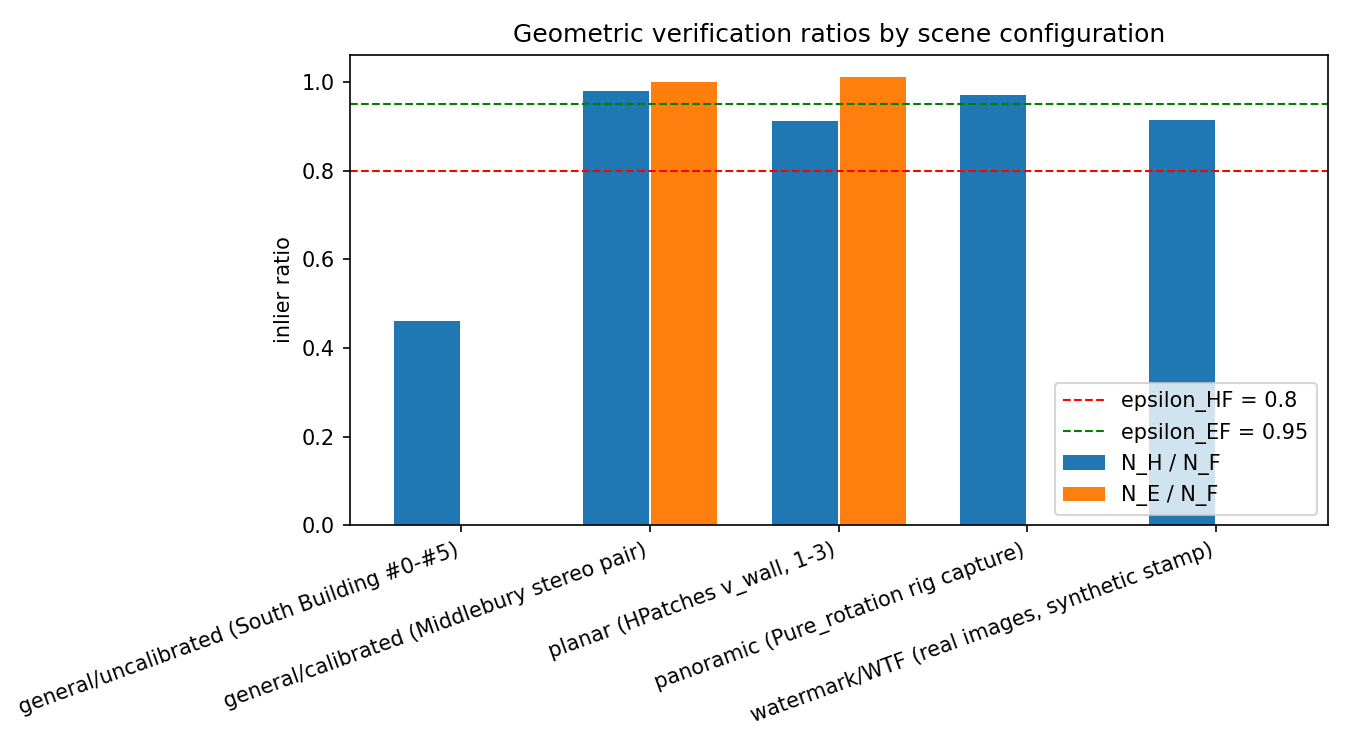
\includegraphics[width=0.7\textwidth]{../results/pair_classification_table.png}
  \end{center}
  \vspace{-0.15cm}
  \begin{center}
  \tiny
  \begin{tabular}{lrrrrc}
    \toprule
    \textbf{Pair} & $N_F$ & $N_E$ & $N_H$ & $N_H/N_F$ & \textbf{Config} \\
    \midrule
    South Building (general) & 26 & -- & 12 & 0.46 & \texttt{UNCALIBRATED} \\
    Middlebury (calibrated) & 1842 & 1845 & 1807 & 0.98 & \texttt{PLANAR\_OR\_PANORAMIC} \\
    HPatches \texttt{v\_wall} (planar) & 492 & 498 & 449 & 0.91 & \texttt{PLANAR\_OR\_PANORAMIC} \\
    Pure-rotation rig (panoramic) & 139 & -- & 135 & 0.97 & \texttt{PLANAR\_OR\_PANORAMIC} \\
    Watermark (real + stamp) & 58 & -- & 53 & 0.91 & \texttt{PLANAR\_OR\_PANORAMIC}, WTF \\
    \bottomrule
  \end{tabular}
  \end{center}
  \footnotesize Only the wide-baseline South Building pair falls below $\epsilon_{HF}=0.80$.
\end{frame}

% ---------------------------------------------------------------------
\begin{frame}{Real-Data Highlight: A Genuine False Positive}
  \begin{columns}[T]
    \begin{column}{0.55\textwidth}
      \begin{itemize}
        \item Middlebury pair has \textbf{real depth variation} --- proven by its shipped
              ground-truth disparity map (\texttt{disp0GT.pfm})
        \item Yet: $H_F$-ratio $=0.98$, $H_E$-ratio $=0.98$ $\Rightarrow$
              \texttt{PLANAR\_OR\_PANORAMIC}
        \item \textbf{Why:} stereo baseline (59.6\,mm) is narrow relative to scene depth
              $\Rightarrow$ a homography fits almost as well as the true epipolar geometry
              at a 4px threshold
      \end{itemize}
    \end{column}
    \begin{column}{0.45\textwidth}
      \small
      This is a real, data-backed instance of Q1's answer: \textbf{a valid H fit is a
      statistical symptom, not proof of true planarity} -- and it directly explains why
      COLMAP treats $N_H/N_F$ as a heuristic, not a certainty.
    \end{column}
  \end{columns}
\end{frame}

% ---------------------------------------------------------------------
\begin{frame}{Experiment 2: Borderline Pair \& Threshold Flip}
  \begin{columns}[T]
    \begin{column}{0.5\textwidth}
      \centering
      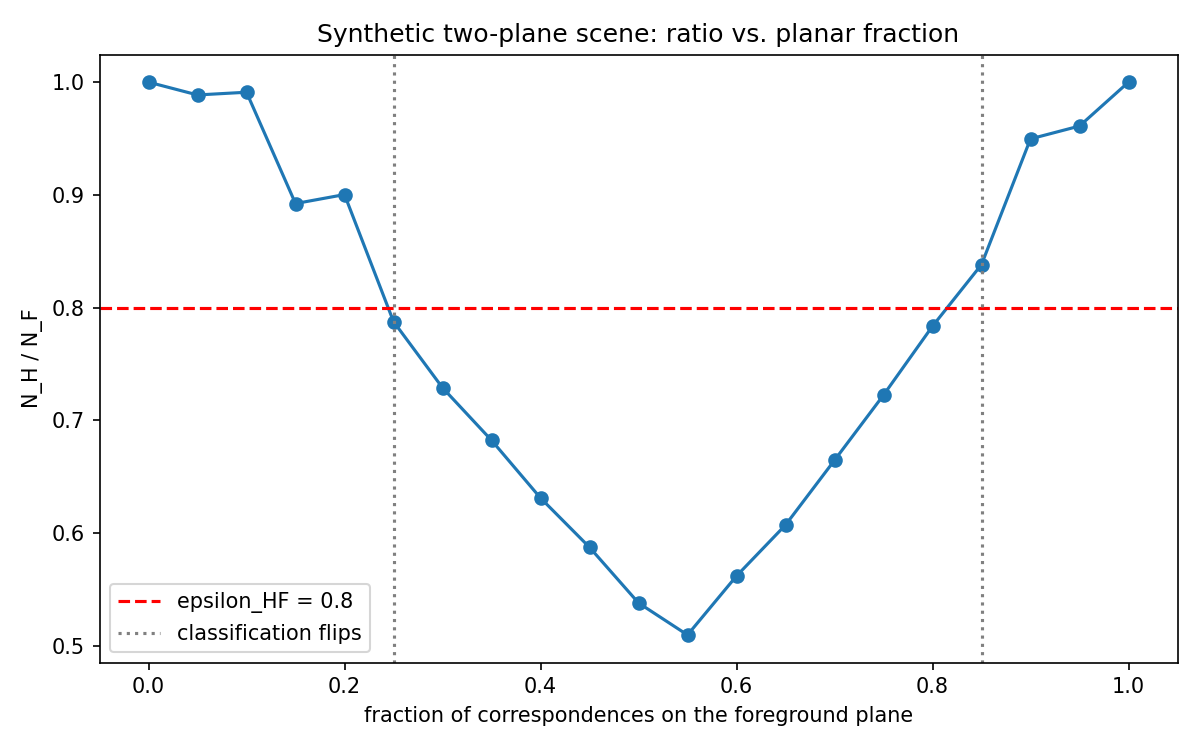
\includegraphics[width=\textwidth]{../results/plane_fraction_sweep.png}
      \scriptsize Synthetic two-plane scene: continuous control of $N_H/N_F$ via the
      fraction of points on one plane. Two clean flips bracket $\epsilon_{HF}=0.80$.
    \end{column}
    \begin{column}{0.5\textwidth}
      \centering
      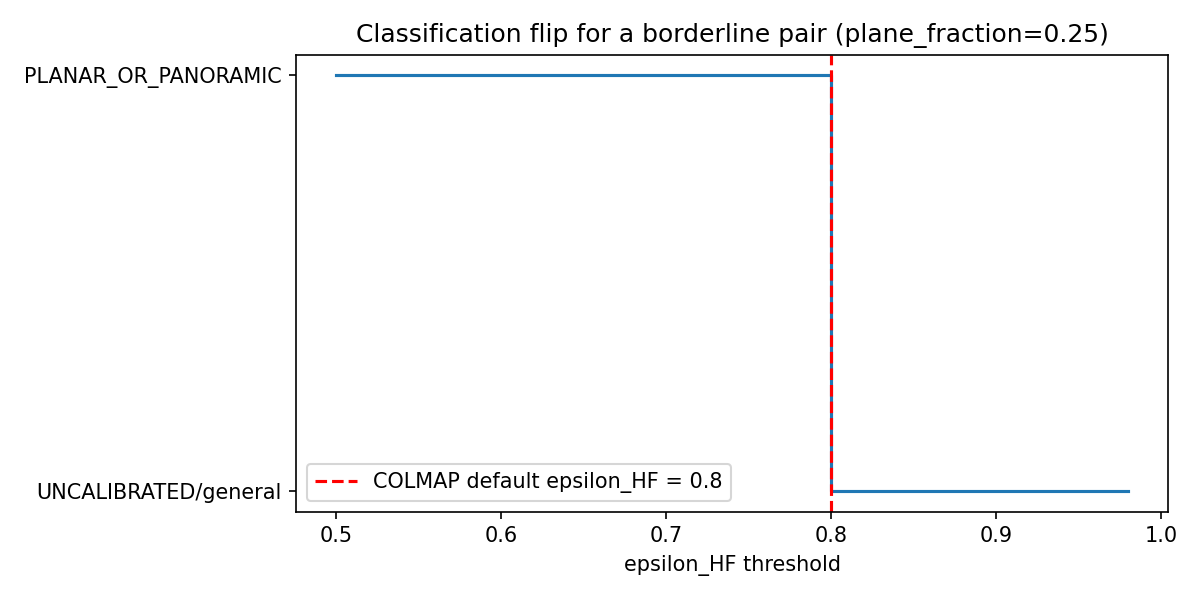
\includegraphics[width=\textwidth]{../results/threshold_sweep.png}
      \scriptsize Fix the pair whose ratio (0.79) sits right next to the real default;
      sweep $\epsilon_{HF}$ itself $\to$ flips exactly between 0.78 and 0.80.
    \end{column}
  \end{columns}
  \vspace{0.2cm}
  Directly answers Q5: a borderline pair's classification is entirely at the mercy of
  where the fixed threshold happens to sit -- there is no soft margin.
\end{frame}

% ---------------------------------------------------------------------
\begin{frame}{Bonus: When Even Self-Calibration Fails}
  Tried to recover $K$ for the panoramic pair from real ground-truth rotations
  ($H = K R K^{-1}$, Hartley \& Zisserman Ch.~8) -- it's provably impossible here.
  \begin{itemize}
    \item Every relative rotation in the rig capture has axis $\approx[0,0,\pm1]$ in the
          camera's own frame: a \textbf{pure roll about the optical axis}, not a pan/tilt
    \item For a roll about the optical axis: $K\,R_z(\theta)\,K^{-1} = R_z(\theta)$
          \textbf{exactly, for every focal length} -- verified numerically to $10^{-14}$
    \item Self-calibration fit confirms it: fitted focal swings from $\sim$50px to
          $\sim$8500px depending on which frame pairs are used, hugging search bounds
  \end{itemize}
  \textbf{Punchline:} a second, independent, data-backed reason (beyond zero baseline)
  the paper never triangulates from panoramic pairs -- this sequence can't even be
  \emph{calibrated} from, let alone reconstructed.
\end{frame}

% ---------------------------------------------------------------------
\begin{frame}{Takeaways}
  \begin{itemize}
    \item Multi-model verification (H \emph{and} F \emph{and} E) exists because
          \textbf{a single model can't tell a genuine general scene from a degenerate
          one} -- F alone can be well-fit even when it's meaningless.
    \item The ratios $N_H/N_F$, $N_E/N_F$ are heuristics against fixed thresholds, not
          proofs -- confirmed by a real narrow-baseline stereo pair being misclassified
          as planar/panoramic despite genuine depth variation.
    \item WTF detection needs a \emph{third}, spatially-localized check (border +
          pure translation) because a translation is a blind spot shared by both H and F/E.
    \item Borderline pairs flip discretely at the threshold -- no soft margin exists in
          this stage of the pipeline.
    \item Panoramic (pure-rotation) pairs are excluded from triangulation for two
          independent reasons: zero baseline, \emph{and} (shown here) the sequence itself
          may not even be self-calibratable.
  \end{itemize}
\end{frame}

% ---------------------------------------------------------------------
\begin{frame}{Backup: Code Reference Index}
  \footnotesize
  All paths relative to \texttt{colmap/src/colmap/}.
  \vspace{0.1cm}

  \scriptsize
  \begin{tabular}{p{4.3cm}l}
    \toprule
    \textbf{What} & \textbf{Where} \\
    \midrule
    Default thresholds (\texttt{TwoViewGeometryOptions}) & \texttt{.../two\_view\_geometry.h:18-111} \\
    Calibrated classification (E, F, H) & \texttt{.../two\_view\_geometry.cc:1075-1235} \\
    Uncalibrated classification (F, H) & \texttt{.../two\_view\_geometry.cc:377-466} \\
    Watermark / WTF detection & \texttt{.../two\_view\_geometry.cc:1550-1615} \\
    Planar vs.\ panoramic split & \texttt{.../two\_view\_geometry.cc:985-992} \\
    \texttt{ConfigurationType} enum & \texttt{scene/two\_view\_geometry.h:16-41} \\
    \bottomrule
  \end{tabular}
  \vspace{0.3cm}

  \textbf{Paper:} Sch\"onberger \& Frahm, \emph{Structure-from-Motion Revisited}, CVPR 2016,
  Sec.~2.1 \& 4.1.

  \textbf{Code \& experiment:} \texttt{problem2\_geometric\_verification/} --
  \texttt{two\_view\_geometry.py}, \texttt{real\_datasets.py}, \texttt{run\_experiment.py},
  \texttt{pure\_rotation\_self\_calibration.py}.
\end{frame}

\end{document}
